\documentclass{article}
\usepackage{amsmath}
\usepackage{graphicx}
\graphicspath{ {images/} }
\usepackage[section]{placeins}
\usepackage{titlesec}
\usepackage{enumitem}
\usepackage{pdfpages}
\usepackage[utf8]{inputenc}
\usepackage{natbib}
\bibliographystyle{acm}
\setcitestyle{authoryear}
\usepackage[hidelinks]{hyperref}

\newcommand{\sectionbreak}{\clearpage}
\titleformat{\paragraph}
{\normalfont\normalsize\bfseries}{\theparagraph}{1em}{}
\titlespacing*{\paragraph}
{0pt}{3.25ex plus 1ex minus .2ex}{1.5ex plus .2ex}

\setcounter{secnumdepth}{4}
\setcounter{tocdepth}{4}

\title{The Lean UX Methodology Application in an Early-Stage Startup: A Case Study of Software Development for Dance Schools Management}
\author{Tomasz Legutko}
\date{Kraków 2017}
\begin{document}

\includepdf[pages={1-2}]{thesis-title-page}
\tableofcontents

\section{Motivation}
Software development methodologies have always been and always will be an important part of all IT projects. With each year, software becomes an even more significant aspect of our society and increasingly, software's complexity becomes harder to manage. A remarkable advancement of architectural patterns, frameworks, tools, best practices and particularly, software development methodologies has occurred over the years.

Historically speaking, software development methodologies have come a really long way from sequential, plan driven strategies to more lightweight, iterative approaches commonly referred to as the Agile methodologies that are nowadays applied by and large in the industry. But as there are no silver bullets, the Agile methods have their limitations and can benefit greatly from extensions.
 
Approaches gathered under the domain of Human-Computer Interface, particularly User-Centered Design were recognized by researchers to be complementary to the Agile shortcomings and there has been a lot of scientific effort put into combining these methods and providing patterns and guidelines for practitioners. 

One important area where these practices cannot be easily applied is startups, that is, newly founded software companies with little to no experience, operating with lack of resources under extreme time pressure to quickly create a product and find an appropriate market for it. To answer the need for a specific approach, Eric Ries proposed the Lean Startup approach.

But as the Agile methodologies could benefit from User-Centered Design practices, so could Lean Startup, and the scientific effort in this area has led to the development of Lean UX approach. Since research on the Lean UX approach is scarce, this study attempts to contribute to the existing scholarship with a case study analysis of a failed startup. The startup aimed to develop software for dance schools management called DNCR and operated from June 22, 2016 to December 1, 2016. The objective of this case study analysis is to evaluate the startup practices in the light of the Lean UX approach and present the findings in order to provide guidelines for industry practitioners.

\section{Introduction}
\subsection{A Brief History of Software Development Processes}
Nowadays, the Agile methods are undoubtedly an IT industry standard. But many view them just as a replacement of the waterfall model, while iterative and incremental development dates back to mid-1950s with a few well-documented undertakings by IBM and NASA \citep{larman2003iterative}.

\subsubsection{The Waterfall Model}
The waterfall model became well-known after Winston Royce's 1970 article "Managing the Development of Large Software System". It promoted a well-defined, strict process, consisting of gathering requirements, analysis, design, coding, testing and maintaining. Even though the original article suggested following these activities twice, the waterfall model was best known as its single-pass version and became a standard for many years to come, especially in large-scale and enterprise projects. \cite{larman2003iterative} argue that, as H.L.Mecken famously said, "For every complex problem, there is a solution that is simple, neat and wrong," the waterfall methodology gave an illusory sense of an "orderly, accountable, and measurable process, with simple, document-driven milestones". It was easy to explain and recall (much easier than iterative and incremental development practices already present at that time) and widely promoted in literature.

\subsubsection{Iterative and Incremental Development Methodologies}
Back in the 1970s, the iterative and incremental development (IID) approach was already becoming recognized as more natural and better fitting for managing projects than the waterfall model; notably, by the IID incorporation in the IBM Trident submarine system with above one million lines of code and in the NASA's space shuttle software. In his 1977 \textit{Software Metrics}, Tom Glib proposed "evolutionary project management" and argued that a system should be implemented in small steps, producing the appearance of stability in order to "have the opportunity of receiving some feedback from the real world before throwing in all resources intended for a system".\citep{glib1977,p.214}

The 1980s brought along vast criticism in literature towards the unquestioned dominance of the waterfall methodology in the industry \citep{larman2003iterative}, advocating the IID approach, with Barry Boehm's notable 1988 publication, \textit{A Spiral Model of Software Development and Enhancement}. It introduced risk assessment and project review in each iteration along with the development phase using an appropriate management model. During that time the US Department of Defense experienced several well-documented significant project failures ensuing from using the document-driven waterfall approach, which resulted in the adjustment of the formal standards (DoD-Std-2167A) to encourage the usage of the IID approach.

By the 1990s, the software development industry became much more aware of the IID practices and many books, articles and standards promoted the IID approach. Furthermore, most of the currently known methodologies: Scrum, eXtreme Programming (XP), Lean Software Development, Rational Unified Process, Dynamic Systems Development Method and Feature Driven Development came into being in the second half of the 1990s.

In 2001, a group of experts representing 17 methodologies, including all of the above, met in Utah to discuss common practices and the term "Agile" was coined.

\subsubsection{Reigns of Agile}

The 2001 meeting resulted in the famous Agile Software Development Manifesto \citep{beck2001Agile}:
\begin{quote}
\begin{enumerate}
  \item Individuals and interactions over processes and tools
  \item Working software over comprehensive documentation
  \item Customer collaboration over contract negotiation
  \item Responding to change over following a plan
\end{enumerate}
\end{quote}

The Agile methodologies clearly promote a lightweight process and have been well received in the industry. They have been increasingly adopted, which is demonstrated by the 11th Annual State of Agile Report in 2017 \citep{one201711th} stating that over 94 percent of over 20,000 respondents claimed their organizations practiced the Agile approach.

Since the creation of Agile methodologies, the industry has also moved forward by leaps and bounds in technical areas. Automation is now common in software processes - quality assurance, continuous integration, continuous delivery and the Internet as development environment, distribution means and execution infrastructure. Not to mention the significant advancement in software languages, tools, frameworks and architectural solutions. \citep{fuggetta2014software}

The progress is unquestionable and although large IT projects were once notorious for spectacular failures (Edward Yourdon's famous \textit{Death March} \citep{yourdon1997death} is a great example of the developing teams' helplessness during a failing project), the reported project success rates (meeting budget and time constraints and project goals) in various studies went from barely 20-30 percent in 2000s \citep{kaur2013software} to 60-70 percent in 2017 \citep{pmi2017pulse}.

\subsection{User-Centered Design}
User-Centered Design is part of the Human-Computer Interaction domain, which primarily focuses on designing and creating interactive systems with the aim to make them user-oriented and usable. It is a very broad domain, focused not only on computer science and engineering, but on incorporating knowledge from various research fields such as cognitive and social psychology, human factors and ergonomics, industrial design and many others. Historically, it has been occupied with the attempts to grasp the nature of human interaction with machines. \citep{ritter2014user}

"System Ergonomics", popular in the 1950s, offered a holistic approach - systems and users were seen as a single interacting system. In the 1960s and 1970s, the "Cognitive Systems Engineering" and "Socio-Technical Systems Design" methodologies were implemented. The Cognitive Systems Engineering approach was an answer to a rapid increase of use and evolution of computer-based technologies, where people's role changed from observing and controlling the machinery and equipment to a very interactive usage. The models were concerned with how people perceive, process and use information to achieve their goals. Socio-Technical Systems Design focused on the interaction between people and technology in workplaces and organizations, trying to optimize the organizational performance and improve humanistic aspects.

Another research area focused on the "Cognitive Modeling". It originated in the late 1950s and its objective was to approximate people's basic cognitive processes and reasoning, explain them and predict how they would evolve under particular conditions. It first centered on how people solve problems symbolically by taking input in a form of symbols, manipulating them and producing output. Later it addressed how information is taken from the external world, especially when using computer systems. The approach then evolved into creating models for human-computer interactions, such as the Human Model Processor, GOMS (Goals, Operators, Methods and Selection rules), Keystroke Level Models and Programmable User Models.

The "User-Centered Design (UCD)" term was coined in 1986 in Norman and Draper's edited collection of essays: \textit{User-Centered System Design: New Perspectives on Human-Computer Interaction}. As \cite{endsley2016designing} states in his book, \textit{Designing for Situation Awareness: An Approach to User-Centered Design}, UCD was an answer to a trend of "Technology-Centered Design", and its key principles were to:
\begin{itemize}
    \item Focus on user's goals, tasks and abilities
    \item Organize technology around the way users process information and make decisions
    \item Keep the user in control and aware of the state of the system
\end{itemize}

In their book \textit{About Face: The Essentials of Interaction Design}, \cite{cooper2014face} discuss a very similar approach: Goal-Directed Design, which primarily focuses also on fulfilling users' goals. In order to achieve this objective, \citeauthor{cooper2014face} provide an in-depth description of research, modeling and requirement gathering activities, focusing on qualitative research, as it allows to create personas representing users. Personas are then used for creation of meaningful context scenarios, which replace traditional user stories. \citeauthor{cooper2014face} also describe the means to define the interaction framework as well as how to validate and iteratively improve it.

A closely related approach of Human-Centered Design considered not only the users' interaction with the system, but noticed the users' human capabilities and limitations and the need to understand them. Examples of the need for such an approach include situations when a user might not directly interact with the system (as in elderly health care monitoring) or when the design needs to incorporate a special consideration for people with some form of disability, e.g. social interaction disorders, such as autism. Human Centered Design is the subject of ISO standard 9241-210, which can be summarized by four main activities:
\begin{enumerate}
  \item Understanding and specifying the context of use (including users, tasks, environments)
  \item Specifying the user requirements in sufficient detail to drive the design
  \item Producing design solutions that meet these requirements
  \item Conducting user-centered evaluations of these design solutions and modifying the design to take into account the results.
\end{enumerate}

Yet another human-centered approach, Design Thinking that first originated in the academic environment in the 1970s, was popularized in the early 2000s by design company IDEO and their CEO, Tim Brown. This approach describes in depth the thought process intended to create solutions that answer user's needs. It consists of five iterative phases \citep{brown2009change}:
\begin{enumerate}
    \item Observe / Empathize - learning about user's values and motivations
    \item Define - developing personas based on user demographics and goals
    \item Ideate - generating ideas with brainstorming and many other practices
    \item Prototype - using low-fidelity methods such as sketches, 3-D models and role-playing to test assumptions
    \item Test - learning what works and what doesn't and iterating based on received feedback
\end{enumerate}
Design Thinking is nowadays often mentioned in reference to human-centered activities. Other popular terms related to this domain include "User Experience" and "Usability". The former is defined as "a person's perceptions and responses that result from the use or anticipated use of a product, system, or service" (ISO 1941-210), but also describes person's beliefs and emotions. The latter is focused on how different tasks in systems are accomplished by users and what errors they make in the process, and so it is often used as interface validation method. 

\subsection{Startups}
Software startups are becoming increasingly popular nowadays. Enormous successes of companies like Facebook, Spotify, Linkedin and many others as well as very accessible technologies encourage many to create their own companies and try to quickly enter the newly emerging markets. These undertakings are of particular interest from the point of view of software process methodologies, as these young companies operate under time and financial pressure to create the right product for the right market in very uncertain conditions. Some of these companies succeed and many fail - in fact, according to the often-quoted statistics, "a great majority of such companies fail within two years of their creation" \citep{paternoster2014software} and "more than 90 percent of startups fail, due primarily to self-destruction rather than competition" \citep{giardino2014early}. As the situation of startups differs from established companies, they require a specialized approach. 

To answer this need, Eris Ries proposed the Lean Startup approach and in his 2011 book defined startup as "a human institution designed to deliver a new product or service under conditions of extreme uncertainty"\citep{ries2011lean}. Steve Blank, who influenced Eric Ries's ideas, highlights three key principles of the Lean Startup method \citep{blank2013lean}:
\begin{itemize}
  \item Instead of creating an intricate business plan based on mostly guesswork, summarize hypotheses in a framework called "business model canvas".
  \item Use Customer Development practices (created by Steve Blank) to test hypotheses - create Minimal Viable Product (MVP) to get feedback from customers and then do Build - Measure - Learn cycles, using metrics allowing for verifying learning and then doing "pivots" if hypotheses turn out to be wrong.
  \item Use the Agile methods to develop MVP. In fact, the Lean Startup is named after the Lean Software Development method, created by \cite{poppendieck2003lean}. This approach was adapted from the Toyota Production socio-technical system and focused on eliminating waste and amplifying learning.
\end{itemize}

Furthermore, Steve Blank argues that among the factors responsible for most common startup failures are the high costs of acquiring first customers, even higher costs of creating the wrong product and too long development cycles. The Lean Startup approach, in his opinion, helps to counter these limitations and make startups less risky. More importantly, the Lean Startup approach is now being taught at universities and is becoming increasingly adopted in the industry.

\subsection{State of the Art}
\subsubsection{The Agile Methodologies}
In recent years, which witnessed a very high Agile methods adoption rate in the industry, it has become clear that the Agile methods are not silver bullets as they have limitations due to organizational and development environments in which they are incorporated. They might be particularly limiting for distributed development environments, large teams and large, complex software \citep{turk2014assumptions}. These findings seem to be consistent with Kenneth Rubith, who in his book about Scrum, the most widely adopted Agile methodology, compared various domains of decision making (using the Cynefin framework) and came to the conclusion that while Scrum was a great fit for the "Complex" domain, it was not the best approach for the "Complicated", "Chaotic" and "Disorder" domains \citep{rubin2012essential}, and the last two are often encountered in the startup environments. However, the Agile methods can be extended to address their limitations. Paradoxically, these extensions are often in the form of practices taken from the more "traditional" development process approaches \citep{turk2014limitations}.

As the Agile practices are now mainstream and have been for a while, they have been very well-analyzed, so research related to them has diverged into many branches. Traditionally, there have been surveys and mapping studies, which have tried to quantitatively measure the trends and answer questions, such as what particular practices are used the most in the industry and in which business domains they are used \citep{diebold2014Agile}. However, most research activity seems to be centered on the intersection of the Agile practices and other, most often the more "traditional" methods.

For instance, \cite{yang2016systematic} studied how to combine the Agile methodologies with Software Architecture, that is, practices related to a high level system design with careful assessment of trade-offs. The Software Architecture practices were initially critiqued for contributing to "Big Design Up-Front" and for leading to excessive documentation and implementation of unneeded features. But the question: "How much design is enough for different classes of problems?" remained unanswered. The architecture design in its early iterations, architecture freeze in the later stages and an iterative delivery of documentation were some of the most representative guidelines identified.

Another example is a study about integrating the Requirements Engineering (RE) methods into the Agile methodologies. Research on the software projects failure rate and factors suggests that among mostly reported failure causes are too much time spent on rework and creating the product out of sync with business, both happening mainly due to poor RE \citep{arcidiacono2017comparative}. RE provides an in-depth description of practices related to requirements elicitation (interviews, focus groups), analysis (prioritization and modeling), documentation and validation (often with prototyping). The Agile RE method differs from traditional RE mostly because of iterativeness - instead of specifying complete specification at the project's beginning, which most often would be unfeasible, requirements are specified iteratively and reprioritized very often (addressing this, Scrum recommends practice called "Backlog Grooming" before every Sprint\citep{rubin2012essential}). An often-faced challenge in the Agile RE approach lies in neglecting the nonfunctional requirements, mainly because customers are for the most part not preoccupied with technical intricacies developers encounter. Other often-reported problems were caused by ignoring the critical aspects,  like scalability and performance at early stages, which inhibited growth later on. Overall, once claimed as heavyweight, the Requirements Engineering approach has found its place in the Agile-dominant industry. Researchers emphasize the importance of "intensive communication between the developers and customers as the most important RE practice". \citep{paetsch2003requirements} \citep{cao2008agile} 

However, by far most spotlight was directed at the intersection of the Agile and User-Centered Design communities.

\subsubsection{The Agile and User-Centered Design Methodologies}
The Agile methodology is now mainstream, but naturally through its focus on a lightweight approach, it does not satisfy all the possible needs. In particular, the Agile community does not extensively discuss users or user interfaces, none of the most often used Agile methodologies include explicit guidance in the area of usability and there is usually no notion of user interface specialists. Generally speaking, the applicability of usability practices in the Agile systems is considered deficient, with the Agile methods focusing primarily on iterative deliveries of working features to customers. Meanwhile, the priority of UCD is user satisfaction, and although there are "philosophical and principled differences between the Agile methods and UCD in focus, evaluation method, culture and documentation", there has been a lot of effort in the community to define practices using both philosophies and they have been referred to as the Agile and User-Centered Design Integration (AUCDI) or, most often, simply Agile UX. \citep{salah2014systematic}\citep{jurca2014integrating}

\paragraph{Agile User-Centered Design Patterns}
The AUCDI patterns use for each stage of Human Centered Design Process ISO 9241-210 standard with an additional step at the beginning \citep{bertholdo2014Agile}\citep{bertholdo2016Agile}:
\begin{enumerate}
 \item Identify Needs for Human-Centered Design
 \begin{itemize}
     \item Sprint Zero
     \item One Sprint Ahead
     \item UX Specialists as Product Owners 
     \item Users time is valuable
     \item Parallel Tracks
     \item UX Specialists as Full-Time Member of the Agile Team
 \end{itemize}
 \item Specify the Context of Use
 \begin{itemize}
     \item Little Design Up Front
     \item Contact Plan of Users
 \end{itemize}
 \item Specify Requirements
 \begin{itemize}
     \item User Stories
     \item More collaboration, less documents
     \item Prototypes as specification
 \end{itemize}
 \item Create Design Solutions
 \begin{itemize}
     \item Low fidelity prototyping
     \item High fidelity prototyping
     \item Design Studio
     \item Collaborative and Participative Design
 \end{itemize}
 \item Evaluate Designs
 \begin{itemize}
     \item Tests with users
     \item Evaluation by inspection
     \item RITE method
     \item Acceptance tests
 \end{itemize}
\end{enumerate}
All stages of the above mentioned patterns should be incorporated for each batch of features in the Agile iteration. These patterns are not meant to be used with great formality, their purpose is knowledge sharing so that teams can select patterns that best fit their specific development environment \citep{bertholdo2016Agile}.

\paragraph{Use of Agile UX in the Industry}
Various reports seem to agree that usability practices in surveyed companies have been increasing in recent years. The most established practices in the industry seem to be Little Design Up Front (LDUF), Sprint 0, designing one sprint ahead and a close collaboration between the Agile and UX teams. In fact, the interaction between the Agile and UX teams has been reported to be the source of most challenges and pitfalls - namely, overworked understaffed UX designers, power struggle with not clearly defined roles of teams as well as work coordination and communication issues. \citep{salah2014systematic}\citep{jurca2014integrating}

As the collaboration between the Agile and UX teams receives most attention in various reports, the "parallel interwoven creation tracks", where the design team works ahead of the implementation team ("one sprint ahead") and uses artifacts as central means of communication seems to be the most recommended approach \citep{brhel2015exploring}. Scrum is seemingly the most fitting methodology for incorporating the UX practices, as teams can plan each sprint together during Backlog Grooming and can both attend daily Stand-Ups. Moreover, a UX member is supposed to be included in a Scrum team on daily basis, as part of the developing team \citep{ovad2015prevalence}.

There has even been created a framework dedicated to integrating usability engineers into an Agile team, called Extreme Scenario Based Design Approach (XSBD), with QXSBD (Quantified) variant, focusing explicitly on the usability-related metrics, but they have yet to receive broad attention \citep{jurca2014integrating}.

\subsubsection{Startups}
Despite the recent years' phenomenon of newly created software companies achieving huge success and wide public attention and recognition overnight, research on this topic is scarce. There is no commonly accepted definition of startups in literature and they are mostly described through the context of their activities, that is, extreme uncertainty (as in \textit{The Lean Startup} \citep{ries2011lean} definition), little to no operating history, lack of resources, intensive time pressure, quick time to market and innovativeness. As a consequence, it is hardly surprising that startups are reported to lack a well-defined processes, but opportunistically select practices when needed, applying the same approach to requirements, documentation, architecture and metrics. Managerial practices are reduced to bare minimum and empowered developers adapt to several roles. \citep{paternoster2014software}

One area of research related to startups focuses on reasons behind a very high startup failure rate. \cite{giardino2014early} attempt to explain failure by performing multiple-case study, analyzing early-stage activities from market, product, team and business perspectives. The most common and costly mistake \citeauthor{giardino2014early} report is startups' focus on technology and developing feature-rich product instead of validating the hypotheses of business idea in the first place, resulting in a working product without customers. The second pitfall is to focus on polished business model allowing to maximize profits before achieving problem/solution fit and addressing the needs of actual customers. Another issue is to neglect the learning process, which results in addressing specific challenges at the wrong time, for example, focusing on improving customer acquisition before receiving feedback from actual users. These mistakes account for a lot of wasted effort, resulting in using up both personal savings for strategy change (or "pivoting", using the Lean Startup terminology) and motivation to run the company any longer. The last factor mentioned as crucial to teams' survival is the "entrepreneur's mindset" of team members, determining their flexibility to handle various, often non-engineering roles as well as highly passionate behavior of founders allowing them to do whatever it takes to overcome countless roadblocks.

The above-mentioned findings seem to be consistent with Steve Blank's, who in his book about Customer Development \citep{blank2013four} suggests putting aside product development in order to test riskiest hypotheses first. It is important to discover and validate problem/solution fit and only then focus on building the right set of features needed by customers, that is achieving product/market fit.

Eric Ries built his Lean Startup methodology \citep{ries2011lean} on top of Blank's ideas. He also admits that startups require appropriate managerial activities and focuses on validated learning (through "build-measure-learn cycles") with usage of proposed set of metrics, preceded by building Minimal Viable Product (MVP) using the Agile methods. In the light of the aforementioned research on startups' failure factors, it could be said that the Lean Startup method addresses them fairly well. Indeed, the method was very well received in the startups community. However, as the Agile researchers have noticed, the Agile methods could be greatly enhanced via practices originated from User-Centered Design, the same can be said about the Lean Startup method, especially since finding the right problem/solution fit is without a doubt tightly connected to understanding and fulfilling users' goals, which is the main area of User-Centered Design interest.

As presented in the previous section, the Agile and UCD integration has been proven to be fairly well researched, so at the first glance it might seem that the problem has already been solved. The main focus of the Agile UX approach, though, is on coordination between the Agile and UX teams, and many startups, especially during the early stages, do not have separate UX teams. Adding startups' pressuring environment and resulting negligence to follow strict processes as well as the need to quickly create different prototypes to find the right problem/solution and product/market fits rather than just focusing on polishing one single product, the guidelines must be adapted accordingly.

To prove this need further, \cite{hokkanen2015ux} provide an interview study with eight startups in Finland and analyze their UX practices. All of the interviewed startups faced challenges in collecting meaningful information from users or customers and did not know how exactly to ask. They did not utilize their user pool due to difficulties with balancing between product development and business creation. Although most of the startups logged user data, they were often unable to extract meaningful information from it. In fact, "they did not have a clear plan on how to collect and analyze the feedback and data".

Recently, researchers have started to explore this area and created a new set of practices and guidelines called the Lean UX approach.
\subsection{The Lean UX Methodology}
\citeauthor{gothelf2016lean}, in their recent book, \textit{Lean UX}, \citep{gothelf2016lean} highlight three foundations upon which the Lean UX methodology is built:
\begin{itemize}
  \item User Experience Design
  \item The Agile Methodologies
  \item Eric Ries's Lean Startup Approach
\end{itemize}
In the area of UX, Gothel and Seiden focus on the Design Thinking approach, which allows to apply design methods to every aspect of business and expand boundaries typically imposed upon designers. In their definition of the Lean UX method, they state, "We work to build a shared understanding of the customer, their needs, our proposed solutions, and our definition of success", which sounds very similar to the User-Centered Design (UCD) related Goal-Directed Design.
\cite{klein2013ux}, in her book, \textit{UX for Lean Startups}, describes how the Lean UX methodology builds upon three foundations:
\begin{itemize}
  \item UCD is enriched by frequent iterations, the Agile teams and validating hypotheses through measuring design outcomes in a scientific manner
  \item The Agile user stories are replaced with user hypotheses that can be either validated or invalidated before being considered "done"
  \item The Lean Startup's hypothesis validation can be designed, performed and interpreted with confidence thanks to provided test strategies and tools
\end{itemize}
Both of the above-mentioned books were first published in 2013, and in the early 2014 Anthony Viviano compiled their basic guidelines into the brief Lean UX manifesto \citep{viviano2014lean}:
\begin{itemize}
  \item \textbf{Early customer validation} over releasing products with unknown end-user value
  \item \textbf{Collaborative design} over designing on an island
  \item \textbf{Solving user problems} over designing the next “cool” feature
  \item \textbf{Measuring Key Performance Indicators (KPIs)} over undefined success metrics
  \item \textbf{Applying appropriate tools} over following a rigid plan
  \item \textbf{Nimble design} over heavy wireframes, comps or specs
\end{itemize}

\cite{liikkanen2014lean} provide an experience report of trying to apply the Lean UX approach in a mid-sized Finnish software company. Major challenges included teaching UI developers user research skills, as they could not afford user researchers in each team and changing the developer's mindset about increments that were no longer defined by implemented features but by hypotheses. Especially since in case of invalidated hypothesis the code needed to be frequently refactored. Other challenges were organizational - outsourcing and distributed decision making (reduced team autonomy) were directly against the Lean UX philosophy of a close collaboration.

Research in this area is still very scarce. The above-mentioned sources, that is, two theoretical books, a manifesto and one brief case study are, as far as is known, the total sum of existing materials on this topic. There is a very clear need for more research on the Lean UX methodology.

\section{Problem Formulation and Methodology}
\label{sec:probl-form-meth}
Taking into consideration the historical development as well as current trends, it becomes clear that the Agile methodologies and User-Centered Design can benefit from incorporating certain aspects of each methodology in their own practices. This area has been thoroughly researched and there are guidelines and patterns to follow.

Despite the recent phenomenon of many successful startups, they have received surprisingly little attention from researchers and because of their unique operating conditions, they require a specific methodological approach. The Lean Startup method addresses many challenges that startups face; however, as in case of the Agile methods, it could benefit greatly from applying the User-Centered Design-related activities. The effort to merge these two domains resulted in the Lean UX approach, but although the theoretical background has been formulated by Gothel, Seiden, Klein and Viviano, there is still very little practical research on the subject.

In attempt to fill this research gap, the present study offers a case study analysis of my own failed startup, which examines the startup's practices in comparison with the Lean UX prescribed guidelines featured in literature.

\subsection{The DNCR Product Vision}
The idea for the project was a two-step vision. The first step was to create a solution for service providers, in that case, dance schools, which would allow to automate and simplify most dance school's business procedures for receptionists and managers, such as calendar management, payment management (online payments and late payers detection), convenient (and mostly automatic) notifications for all course attendees and client history, profiles and statistics, which would improve business and marketing capabilities of dance companies. The product was named "DNCR" (pronounced "dancer").

The second step was focused on service recipients, that is, dance classes attendees. The main idea was to create a search engine integrated with DNCR, so that all schools using DNCR could easily provide an always up-to-date schedule. Moreover, users could quickly compare dance schools and courses to find the exact dance class they need and enroll, handle payments online and review the course, school and instructors later. This way DNCR would become not only a business process support service for dance schools but also a great opportunity to access a pool of potential new clients.

This idea could later be expanded in various ways, depending on what would be of most value to customers, with possibilities from building a dance-oriented community to adapting the solution to solve similar problems in numerous other domains, such as fitness and wellness centers, language schools and so on.

Dance schools were chosen as a primary target as they represent a narrow-enough market to solve their exact, specific problems, which was small-enough so there would not be many existing specialized solutions (market was not saturated). Moreover, a few of the co-founders were either active dancers or have attended dance classes in the past, so they already had some domain knowledge and contacts with dance schools. Further activities were performed later on in order to validate the problem the team was trying to solve, including qualitative and quantitative market and competition solutions research. These are described in more detail in Section \ref{sec:dncr-project}.

\subsection{Methodology}
In order to answer research questions, a case study analysis is presented in order to examine the decisions and progress made by the startup developing the DNCR project from June 22, 2016 to December 1, 2016, when the startup was disbanded, failing to complete the Minimal Viable Product and reach the market.

In his book, \textit{Case Study Research}, \cite{yin2013case}, lists five rationales for a single-case study design and the DNCR project case study fulfills three of them:
\begin{itemize}
\item \textit{Representative or typical case} - each startup is undoubtedly a unique undertaking, but the DNCR project team was quite representative for a startup, demographically speaking: it consisted of mostly students finishing or having just finished their graduate IT studies, with some work experience and no previous startup experience
\item \textit{Revelatory case} - as mentioned during state of the art discussion, there is hardly any research on attempts to apply the Lean Startup method and virtually no research analyzing startups in the light of the Lean UX approach
\item \textit{Longitudinal case} - Yin defines longitudinal case as "studying the same single case at two or more different points in time" – this startup is analyzed at three different points in time: 1) during the first five months of startup development activities, 2) on the final day of the startup (incorporating the conclusions the team had on the day of ending the project) 3) a few months later, a retrospective examination, enriched by insights from literature.
\end{itemize}

Furthermore, using Yin's terminology, the case study can also be described as \textit{holistic} (as opposed to \textit{embedded}), because it focused on the team as a whole without involving several units of analysis (i.e. the study did not focus on analysis and comparison of individual developers in the team).

\subsubsection{Methodological Limitations}
Christine Meyer \citep{meyer2001case} argues that although a "longitudinal study enables one to track cause and effect, [it] can make one aware of intervening variables", allowing one to see and understand the context more clearly, it may also be a subject to significant research biases:
\begin{quote}
In a real-time longitudinal study, the researcher is in danger of losing objectivity and of becoming too involved with the organization, the people, and the process. Hence, Leonard-Barton (1990) claims that one may be perceived as, and may even become, an advocate rather than an observer.
\end{quote}

Moreover, there are common misconceptions about generalizability of single-case studies and validity of achieved conclusions.

\cite{flyvbjerg2006five} addresses both researcher bias and generalizability objections. Arguing against the former, Flyvbjerg notes that many experience reports lead to a belief that researchers are usually aware of this tendency and as a result "it is falsification, not verification, that characterizes the case study" and there is no greater bias than in any other scientific method. Flyvbjerg addresses the latter arguing that "formal generalization is overvalued as a source of scientific development" and that context-dependent, concrete knowledge is even more valuable than "predictive theories and universals".

Discussing generalizability, \cite{meyer2001case} expresses the need for a balance between in-depth, longitudinal studies providing a possibility to make judgments about applicability and greater generalizability offered by multi-case approach. Moreover, she notes that "generalisation is about theoretical propositions, not about populations".

Further discussing the case study limitations, \cite{yin2013case} argues that a holistic case study can suffer from a "shift of case study nature" during the course of study, which may impact both initial approach and initial research questions. This, according to Yin, is the source of the greatest criticism of case studies, although, as assumptions change and new questions emerge, this flexibility can also be considered a strength.

This shift has certainly taken place during the DNCR project, because due to the project failure, the discussion about methods applicable in a startup's lifecycle can only focus on the early-stage startup activities. This means that many important aspects of the Lean Startup methodology, most notably qualitative metrics such as A/B testing allowing to test hypotheses about developed product, cannot be discussed, as the startup did not survive long enough to implement and use them. However, an analysis of factors leading to an early failure has proven to be illuminating on its own.

\subsection{Research Questions}
In methodological assessments of software projects in recent literature, there has been a general tendency to divide project activities into several categories.

In their multiple-case study of an early-stage startup failure analysis, \cite{giardino2014early} propose four dimensions of evaluation, drawing upon the study of \cite{macmillan1987criteria}: team, product, business and market.

Based on their systematic literature review of the Agile and User-Centered Design integration,  \cite{brhel2015exploring} propose a coding system to group all relevant aspects into four main categories: process, practices, people/social and technology.

In \textit{A survey study of critical success factors in Agile software projects} \cite{cao2008agile} at first present five dimensions most recently used in literature in failure/success research: organizational, people, process, technical and project. Then, based on their hypothesis testing result, \citeauthor{cao2008agile} list six success factors, presented from the most to least significant: delivery strategy, Agile software engineering techniques, team capability, project management process, team environment and customer involvement.

Drawing upon the above proposed categories and including the Lean UX specific questions, this case study analysis will address the following research areas about the early-stage startup activities:

\begin{itemize}
\item[RQ1:] Which Lean UX practices are most important in the early stages of a startup?
\item[RQ2:] How can Lean UX practices influence Minimal Viable Product building and what are the impediments in adopting them?
\item[RQ3:] What are the key challenges in startups regarding technology?
\item[RQ4:] What are the factors that impact the success of startups regarding team?
\item[RQ5:] Which Lean UX practices can be used in startups regarding business/market?
\item[RQ6:] How are success factors in Agile projects \citep{cao2008agile} applicable to startups?

\end{itemize}

\section{The DNCR Project: An Overview}
\label{sec:dncr-project}

\subsection{The Commencement of the Project}
The project began on June 22, 2016, when one of the co-founders brought the idea for the project along with its first client to six other developers (all seven developers had months of experience working in the same company). The idea was then refined and basic working rules were set, concerning the distribution of profits and amount of working hours spent each month - one person worked full-time, six others agreed to work for \( \frac{1}{4} \) - \( \frac{1}{5} \) full-time equivalent along with their current jobs. The team decided to focus on the Krakow and Silesia regions, where many dance schools they were familiar with were located.

A week later the team created a Minimal Viable Product (MVP) vision along with the initial list of requirements, revolving mainly around basic dance courses, attendees, instructors and payments management and email notifications. The team considered it the most basic "notebook replacement" version and scheduled the date of the first release for October, 2016, when the academic year starts, since students were one of the main targets of the dance schools and most courses would start then.

\subsection{Sprint 0: Market Research}
During the first month, the team only knew they had one customer in need for their solution, and they needed to know a lot more.

\subsubsection{Quantitative Local Market Analysis}
The first step was to approximate the size of the targeted market and to have a better understanding of the currently used solutions. In order to do that, the team analyzed websites of all dance schools in the region and estimated their size, website and schedule quality and ability to enroll online. The findings were promising: out of 35 dance schools in Krakow and 45 in Silesia only 8 had websites without schedules, 13 had no dedicated websites and only 10 allowed some form of online enrolling (usually via a non-interactive html form). The existing sites and schedules were mostly of poor quality and none of the websites offered an online payment possibility.

Another aspect of quantitative research that was conducted entailed an online distributed survey for dance classes attendees. Out of 37 respondents, most were very enthusiastic about a possibility of online payments (60\%) and an ability to compare courses and schools online (60\%) and dissatisfied (70\%) with their schools' current schedule management. Among other problems encountered with the schools, the respondents pointed out the inability to pay in a form other than cash and the lack of notification when a class was rescheduled.

\subsubsection{Qualitative Local Market Analysis}
Another step, performed simultaneously with the previous ones, was in accordance with the Lean Startup strategy to "Get Out Of The Building" and talk to potential clients. Qualitative, in-depth interviews were carried out with potential clients: one initially interested client from Kraków and his two receptionists and with one potential client from Silesia. Another two, more brief interviews, were performed with two additional schools. The purpose was to identify the currently applied solutions (mostly paper notes + Excel or huge ERP system) and their limitations. Several factors were discovered, and the bottom line was that the team's initial system vision seemed to be the right direction to take. Both in-depth interviewed schools had problems with late-payers and were not satisfied with their current solutions.

\subsubsection{Competitive Products Audits}
The team was initially aware of only two related products. One was the loyalty program software the first client was about to buy and the other was complex club management software for large fitness centers. The team soon reviewed the demonstration versions of both applications, evaluated them and their target markets, and concluded that they were not direct competition, but many things could be learned from them (both in terms of business and user-interface).

Afterwards, a more detailed competitive products analysis was performed, and the scope was extended to gym and fitness centers management software, 41 solutions (including the ones mentioned above) were found, operating mostly in the US. Out of them, nine demonstration versions were reviewed. Several similar markets were identified (individuals needing to manage their schedules and let clients make appointments online, solutions for ballet dance companies which help to organize ballet performances and complex solutions that worked for both dance companies and fitness / spa / wellness / yoga and other similar domains). Some of these products boasted tens of thousands of cooperating companies, so the main takeaway was that if there was such a huge demand outside of Poland, then there should be a great local market opportunity waiting to be explored.

Nine of the identified solutions offered products in Polish, but they were mostly targeted at gyms and fitness centers. One direct competitor that focused on dance schools was identified, providing most of the intended DNCR features, but they were not actively marketing their product and expanding aggressively. Having evaluated their demonstration version, the team decided that there were many ways the experience could be improved.

As far as the dance course search engines go, there were two sites attempting to aggregate dance school and allow to search among them, but they both had the same problems - they featured very outdated data, inserted manually some time ago, poor searching capabilities and seemed to be more or less abandoned. The DNCR solution, as previously mentioned, would integrate with search engine, so that data would be always up to date. There is a capable search engine for Benefit Multisport Card customers, popular and honored card among the local dance schools, but its main problem is limitation to their customers. Some foreign search engines were identified, but they all limited their results to their chains of dance schools. The dance attendees survey showed that there appeared to be two most popular ways to search for dance courses online - via Facebook or Google, but although Google provides a nice visualization on the map and some opinions, whereas Facebook provides likes and reviews, neither of them offers an in-depth comparison of courses, with regard to their type, dates, required skill levels, etc.

\subsubsection{Market Research Conclusion}
The team performed both qualitative and quantitative market and competition analysis and was confident that there was a market opportunity to explore, especially considering the demand for solutions outsides of Poland. Evaluating many related existing solutions allowed to explore many ways to implement business model (i.e. pricing and payment options), business domains to explore and user interface ideas and shortcomings. The team started drafting a business model document, and simultaneously to research and implementation efforts, the team looked for a way to legalize their company.

\subsection{Sprint 0: Architecture and Technologies}
The team consisted of six developers who worked on the desktop Java application on a daily basis and one developer experienced with PHP and web technologies. The architecture was pretty standard these days: it was decided that the DNCR would be a web app with a server, as it would be easiest to distribute and quickly introduce new changes, as well to introduce a web search engine later on.

For the front-end, the team decided to create a Single-Page-App (SPA), as there were many frameworks with great support that would facilitate learning. Despite Facebook React's vast popularity, the team decided on the Angular framework from Google (despite it being beta before 2.0 version at that time), as it seemed more opinionated and provided a more complete, all-in-one solution that would be the easiest to grasp by the team consisting mostly of developers inexperienced with web technologies. Typescript was chosen instead of Javascript, as it was both promoted by Angular and the team used to static typing was enthusiastic about retaining some typing capabilities.

For the back-end, after initial research of server and maintenance costs, as well as a seemingly uncomplicated server-side logic, Java was quickly ruled out. Initially, the team decided to choose Ruby on Rails, due to inexpensive costs of server maintenance and expressive language, but as no one on the team had experience with this language and its frameworks, the decision was made to use PHP instead, along with Laravel 5 framework and have at least one expert on the team.

As for the database, the model was characterized by relations between course attendees, courses, payments, instructors and course dates, so it could be naturally modeled with relational database, so the team picked MariaDB. It was accessed using Laravel Active Record ORM - Eloquent. The schema, created a little bit later, is presented in Figure \ref{fig:schema}.

\begin{figure}[h]
    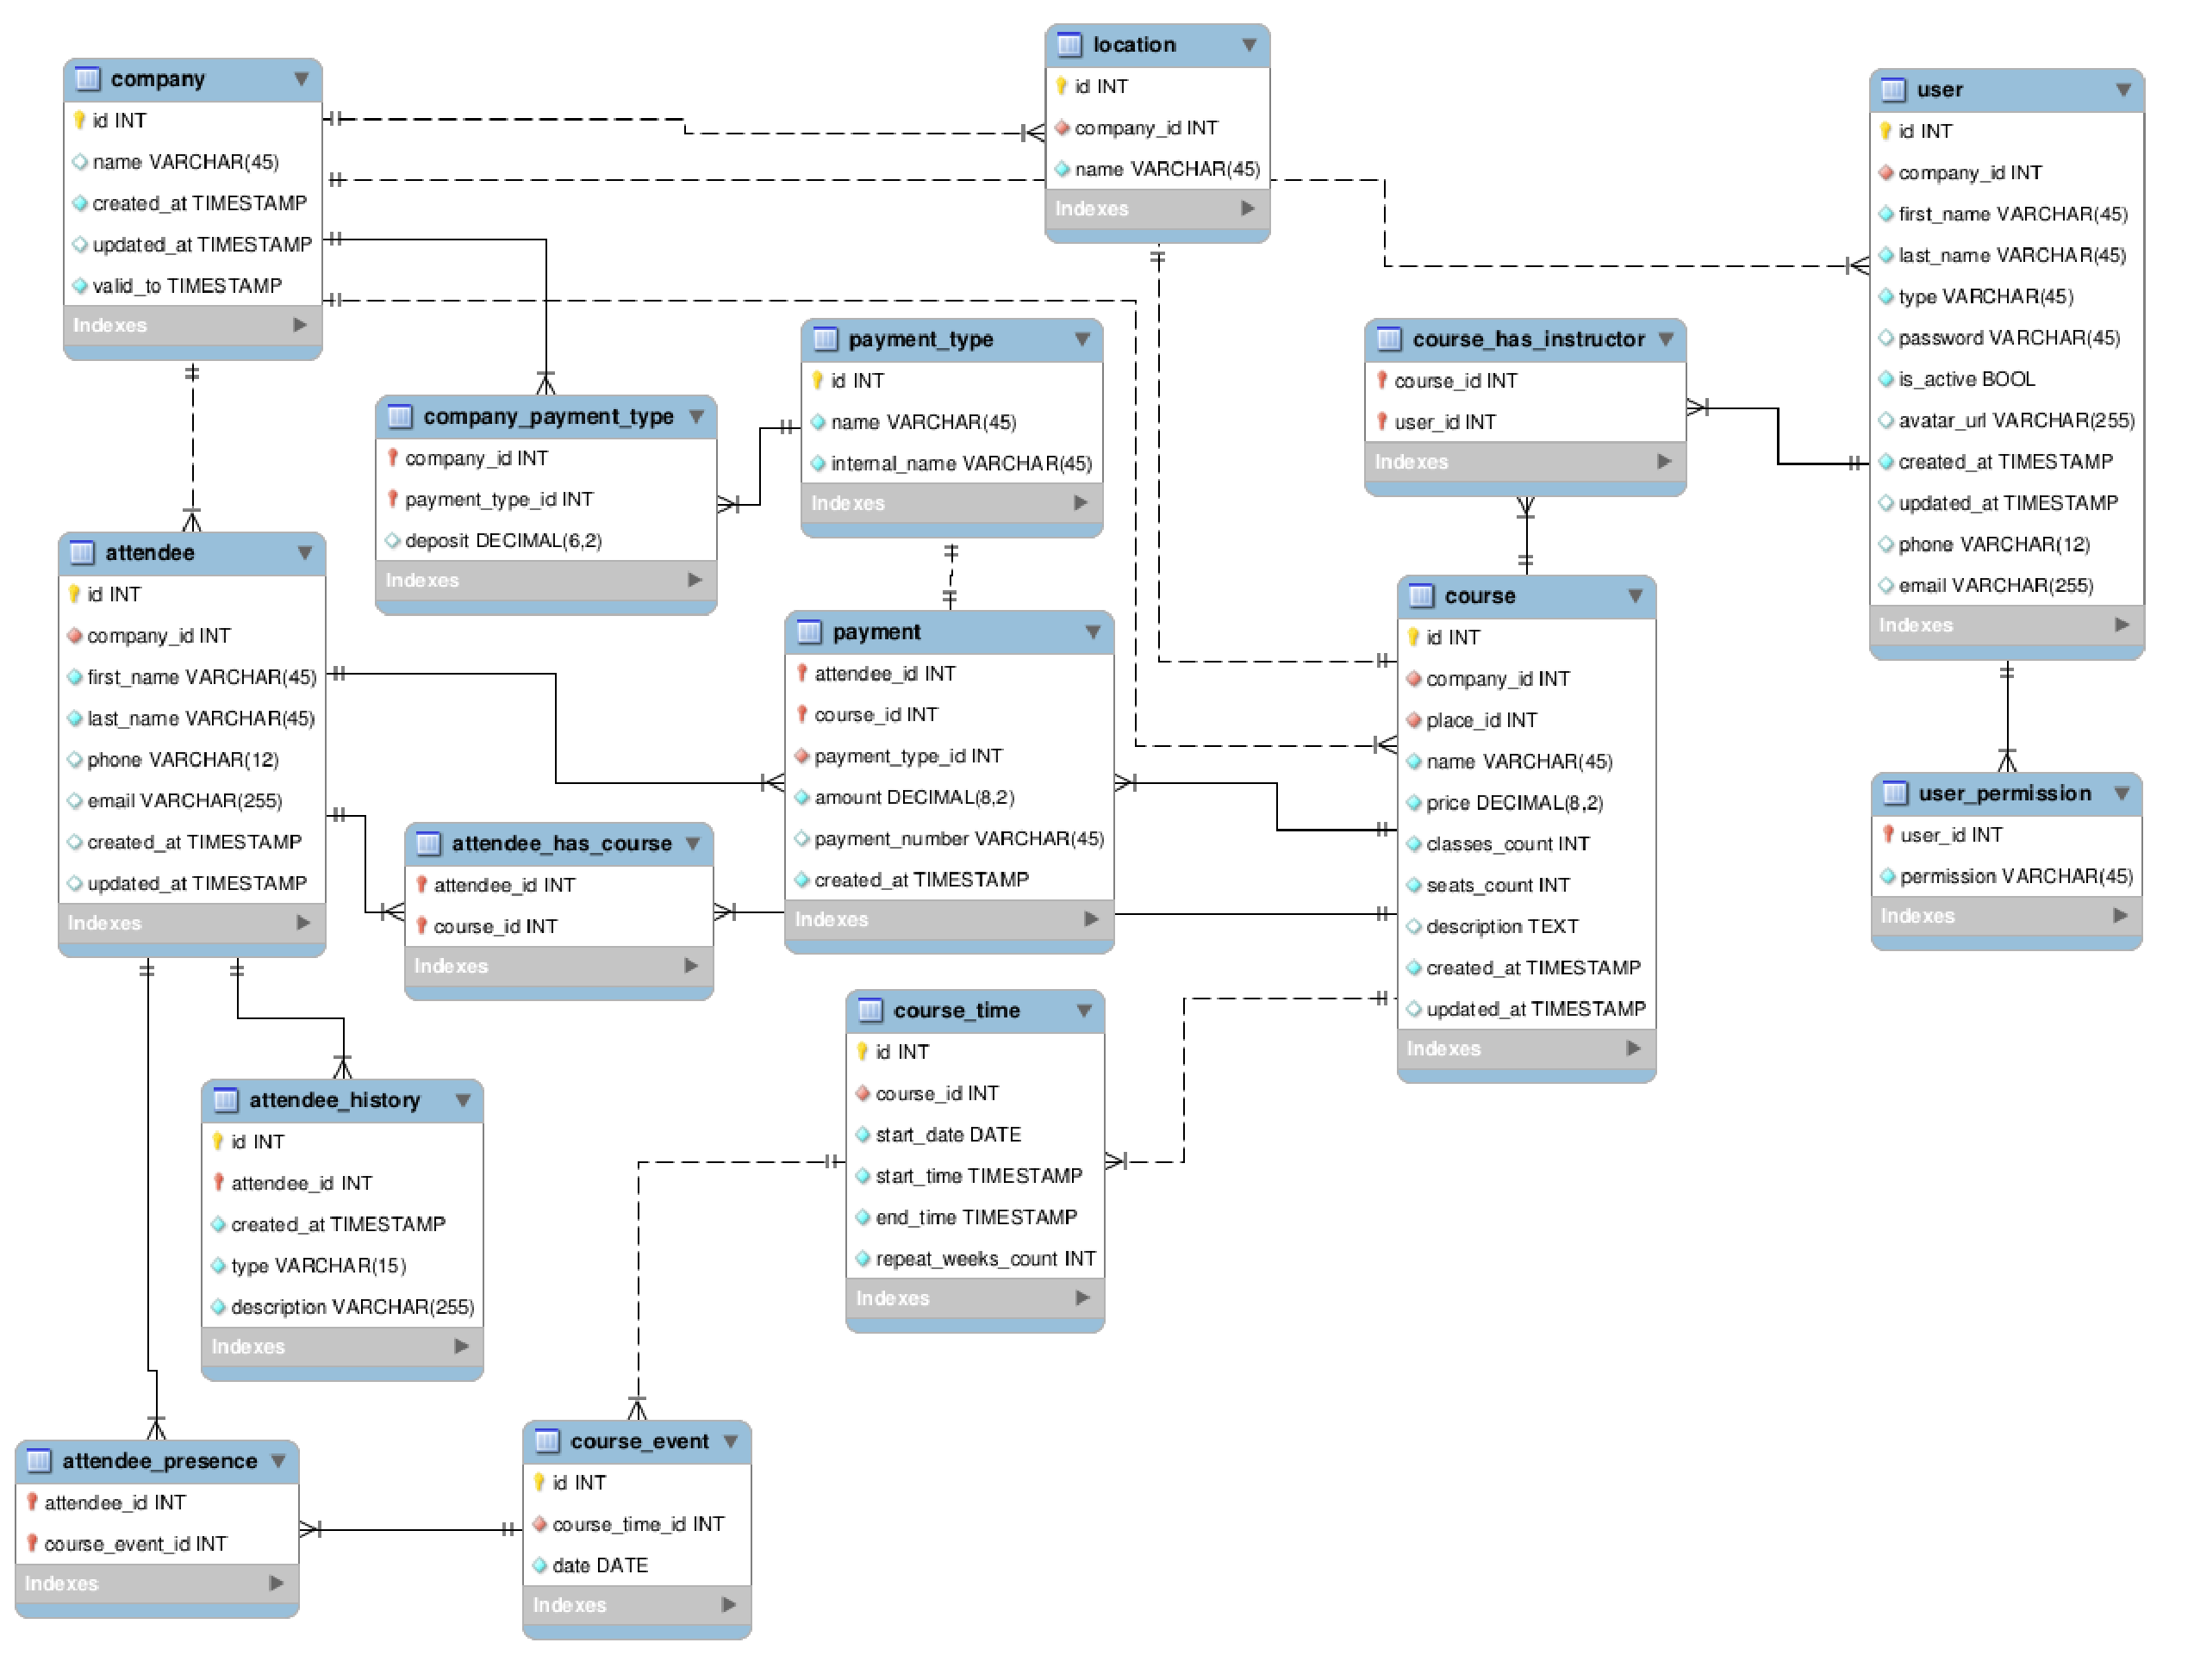
\includegraphics[width=\textwidth]{schema}
    \caption{The schema of the DNCR database presents relations between dance school (company), courses, attendees, payments and instructors / administrators.}
    \label{fig:schema} 
\end{figure}

Another decision was made to use lightweight virtualization for the development environment. The team used Docker containers to achieve the same environment as on their server, i.e. Debian with Apache configured to serve both the minimized Javascript front-end app and handle API calls to backend PHP app. This way, despite working on different operating systems, the whole team would have the exact same server environment with the same dependencies and versions of each library and tool. Another, very similar Docker image was used for Continuous Deployment, that is, after each Pull Request tests were launched inside Docker image using Shippable DevOps platform in order to ensure that application would not break in some unexpected way.

For an easy collaboration, the team initially used Asana, but after a month switched to Trello to manage amount of work in progress (WIP) via Kanban board. For Git, private GitHub repository was used and all the tools were integrated with instant messaging tool, Slack.

\subsection{Next Sprints: Focus on Implementation}
After market research to gain confidence in the initial direction of the project was carried out, technological decisions were made and the developer environment was all set up, in late July the team decided to focus all efforts on implementation in order to have the MVP ready for October.

By this point in time one of the team members had to resign due to personal reasons, but other six developers looked optimistically towards the implementation phase.

\begin{figure}[h]
    \includegraphics[width=\textwidth]{gui-sketch}
    \caption{A low fidelity GUI sketch presenting calendar and selected course in single view}
    \label{fig:gui-sketch}
\end{figure}
\begin{figure}[h]
    \includegraphics[width=\textwidth]{gui-balsamic}
    \caption{A high fidelity GUI prototype using Balsamic program, same view as presented in Figure \ref{fig:gui-sketch}}
    \label{fig:gui-balsamic}
\end{figure}
\begin{figure}[h]
    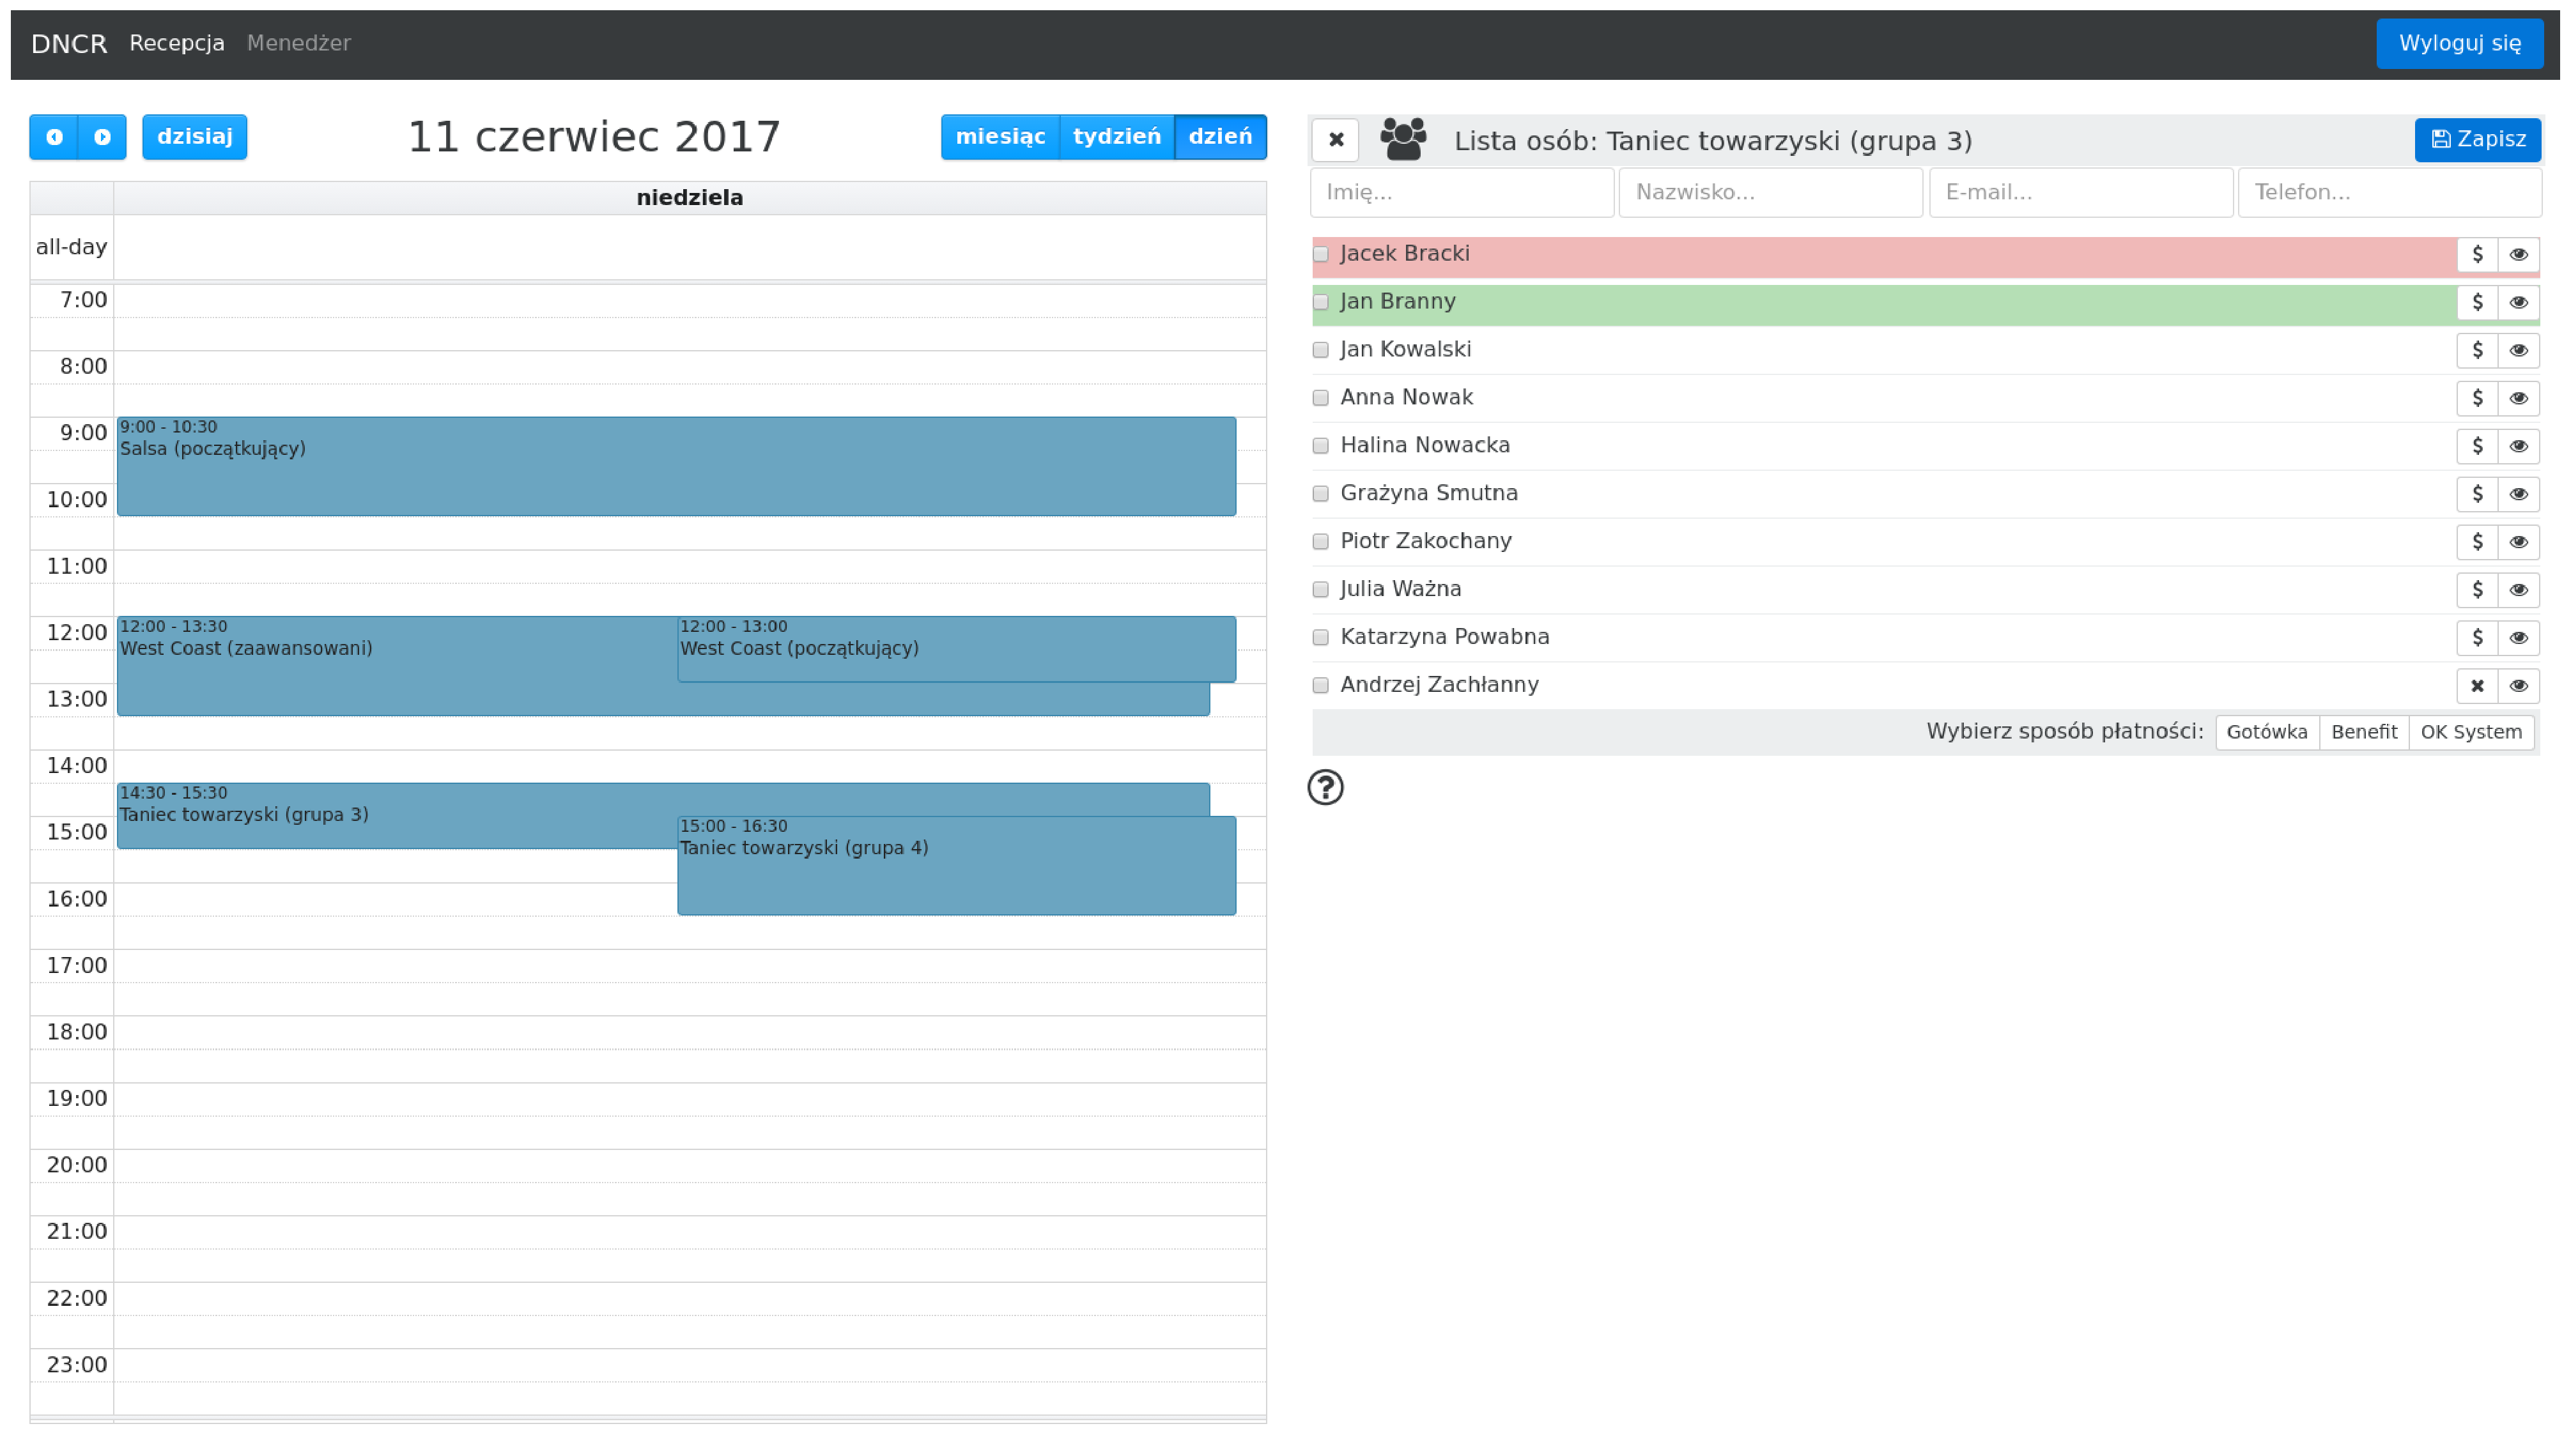
\includegraphics[width=\textwidth]{gui-angular}
    \caption{An actual application in Angular, same view as in Figures \ref{fig:gui-sketch} and \ref{fig:gui-balsamic}.} 
    \label{fig:gui-angular}
\end{figure}

\subsubsection{Mockups and GUI Vision}
The Graphical User Interface (GUI) was a very important aspect of the project because one of the main problems to be solved was the elimination of manual and repetitious actions that had to be performed by a dance school receptionist. The team aimed to make the user interface easy and convenient. It was clear from the beginning that the interface would evolve around a calendar view. At first, the team discussed the GUI using a low-fidelity sketch on paper, and then, for an implementation reference as well as for a GUI validation with the client, a high-fidelity GUI prototype was prepared using the Balsamic program. Figures \ref{fig:gui-sketch}, \ref{fig:gui-balsamic} and \ref{fig:gui-angular} present the same view evolution from a low-fidelity sketch to the actual application.

\subsubsection{Client Meeting and Design Validation}
On August 12, the team representatives met with a client to verify the created design. The client was shown an interactive prototype achieved through the use of Balsamic Links, i.e. buttons on static wireframes linked to other static wireframes, producing an illusion of full interactivity. The client found the prototype to his liking and was satisfied with the simplicity of the design. He then suggested an incorporation of various additional features in the later phase of the project, such as different client types and an award system (features from the loyalty program software he was familiar with), integration with his school's website, attendance visualization and checking attendance via QR-codes or a special electronic card. After the discussion, it was agreed that after the MVP was completed, the idea of adding these features would be revisited.

% \FloatBarrier
\subsubsection{The Collaboration Model}
The team decided that all six developers on the team would be working "full-stack", that is, both on the back-end and front-end sides of the app so that each developer would have a sufficient autonomy in order to quickly implement full business features. As mentioned earlier, only one developer had been previously acquainted (and in his case, proficient) with the used technologies. The team accepted an initial slow-down for everyone to learn the technologies and predicted to gain traction after a few weeks.

As most of the team worked only part-time on the project and the team naturally did not have a dedicated workplace for their needs at that point, four team members agreed to work daily in the morning at an agreed time before work - 7:00 a.m., while two other members preferred later hours. The goal was to minimize the feedback-loop between team members, so each question / interaction / review would not have to wait a few days for response, unnecessarily prolonging the completion of each task. Moreover, the team decided to meet every month to discuss progress, areas to improve and the general direction and strategy.

\subsubsection{Sprint 2: Implementation Progress (August)}
In August, the first features of the project began to appear:
\begin{itemize}
\item The login page
\item An initial, basic version of the landing page in order to promote product
\item Basic manager (admin) and receptionist views
\item Adding new attendees
\end{itemize}
Furthermore, the database schema was created and online payment intermediaries research was performed in order to prepare the ground for the possibility to pay for the courses online.

By this time, it became clear that working remotely proved to be a bigger challenge than the team expected. Only two members of the team worked regularly each morning as was agreed on and two members did not make progress on any task.

\subsubsection{Sprint 3: Implementation Progress (September)}
The following features were implemented in September:
\begin{itemize}
\item The login authentication
\item An attendees list view
\item Adding dance instructors and instructors list view
\item A calendar component presenting courses
\end{itemize}
It is worth noting that all of the above-mentioned tasks fell under a very broad definition of "done". Each task included the front-end and back-end validation, handling different sizes of display (via Bootstrap framework responsive capabilities), and even an elegant back-end internationalization, which resulted in very long implementation and review periods. The implementation of some tasks took a few weeks and then it took a few additional weeks to thoroughly review them.

It started to become clear that the MVP by October was out of the question. The team decided to focus less on polishing of the product and to start creating more granular tasks, so new features could be added more quickly. Another enthusiastically received idea was to create "hackatons", that is, long whole-team programming sessions, where one technology experienced developer would coach others in their work.

\subsubsection{Sprint 4: Implementation Progress (October)}
The October progress:
\begin{itemize}
\item A dance course creation
\item The attendee details / profile view
\item The authorization feature improvement: an automatic token refreshing so that a user would not be logged out during the application usage
\end{itemize}

Despite numerous discussions on task implementation taking too long in the previous month, in October the problem worsened due to an even less regular working schedule combined with the inability to schedule "hackatons". Consequently, motivation was plummeting and the team members were clearly not spending the promised amount of time working on the project. An intervention was needed and in order to improve work consistency, motivation and to increase morale, the team decided to log worked hours and change ad-hoc "Stand-ups" (officially called "Daily Scrum Meetings" held to summarize work progress and discussion of eventual impediments) to obligatory weekly "Stand-ups" where each team member would present their weekly work log.

\subsubsection{Sprint 5: Implementation Progress (November)}
The following features were implemented in November:
\begin{itemize}
\item Multi-tenancy - the application could now handle multiple dance schools 
\item Payments - a receptionist could insert an attendee payment with one of several available methods
\item Application-wide notifications
\item Mail tool for communication with attendees
\item A visual indication of an attendee payment status
\item Dance course editing and handling multiple course times
\end{itemize}
Although the features implemented in November might indicate progress, in fact, most of them were just a result of implementation efforts made during the month of October. In November, the feature-creation cycle took even longer and work-logging and weekly "Stand-ups" were of little help, as most members spent less and less time on the project.

\paragraph{Meeting with a Subject Matter Expert}
On November 12 a team representative met with a subject matter expert, a senior ballroom dancer who organized dance tournaments, was knowledgeable about the target market and had collaborated with various dance schools. 

The first part of the meeting consisted of a loosely designed usability test: the expert saw the application for the first time and knowing the objective of the application, he was supposed to discover the application capabilities by himself without any guidance. His interaction was observed and all remarks and troubles were recorded.

As a result, eighteen improvements were suggested and discussed, ranging from major usability flaws like the inability to add an existing attendee to another dance class (the GUI for adding attendees to a course only allowed for creating new ones) to various features the team had not yet considered, but which were an integral part of the schools' business procedures, e.g., how to handle "waiting lists" when a dance class reached the participants' limit or someone waited for the course to start in the future? Would the registrants be considered as enrolled in a course after they expressed interest and provided their data, or only after they submitted the payment? How to handle bonus visits and coupons for clients who could attend several classes in a given course? How to handle courses designed "for couples" only? And many other similar aspects not previously considered.

During the second part of the meeting, the business model was discussed, in particular the online payments viability for dance schools and due to various legal reasons (i.e. fiscal evidence), it was decided to postpone the development of this feature and to substitute it with a plain email reminder about due (or upcoming) payments with the dance schools' bank account information, as an easier way to validate the idea with fewer legal consequences.

\subsection{The Decision to End the Project}
Eventually, after a consultation with each team member about their individual reasons for the constantly decreasing commitment, during a meeting on December 1, the decision was made to end the project. The team decided to open-source the code on GitHub (\url{https://github.com/tlegutko/dncr}), the client would be offered a possibility to evaluate competitive software and the team did a "Project Retrospective" to discuss what went well and what lessons were learned.

The team's December discussion and conclusions are presented in Section \ref{sec:dncr-proj-eval} as part of the project evaluation.

\section{The DNCR Project Evaluation}
\label{sec:dncr-proj-eval}
This section begins with the project evaluation performed by the whole team on the day the project ended and proceeds to address the research questions specified at the end of Section \ref{sec:probl-form-meth}.

\subsection{The DNCR Retrospective Meeting}
The whole team met on December 1 and made the decision to end the project. Then the team proceeded to do a "project retrospective" in order to discuss strengths and weaknesses of the project.

\begin{figure}[h]
    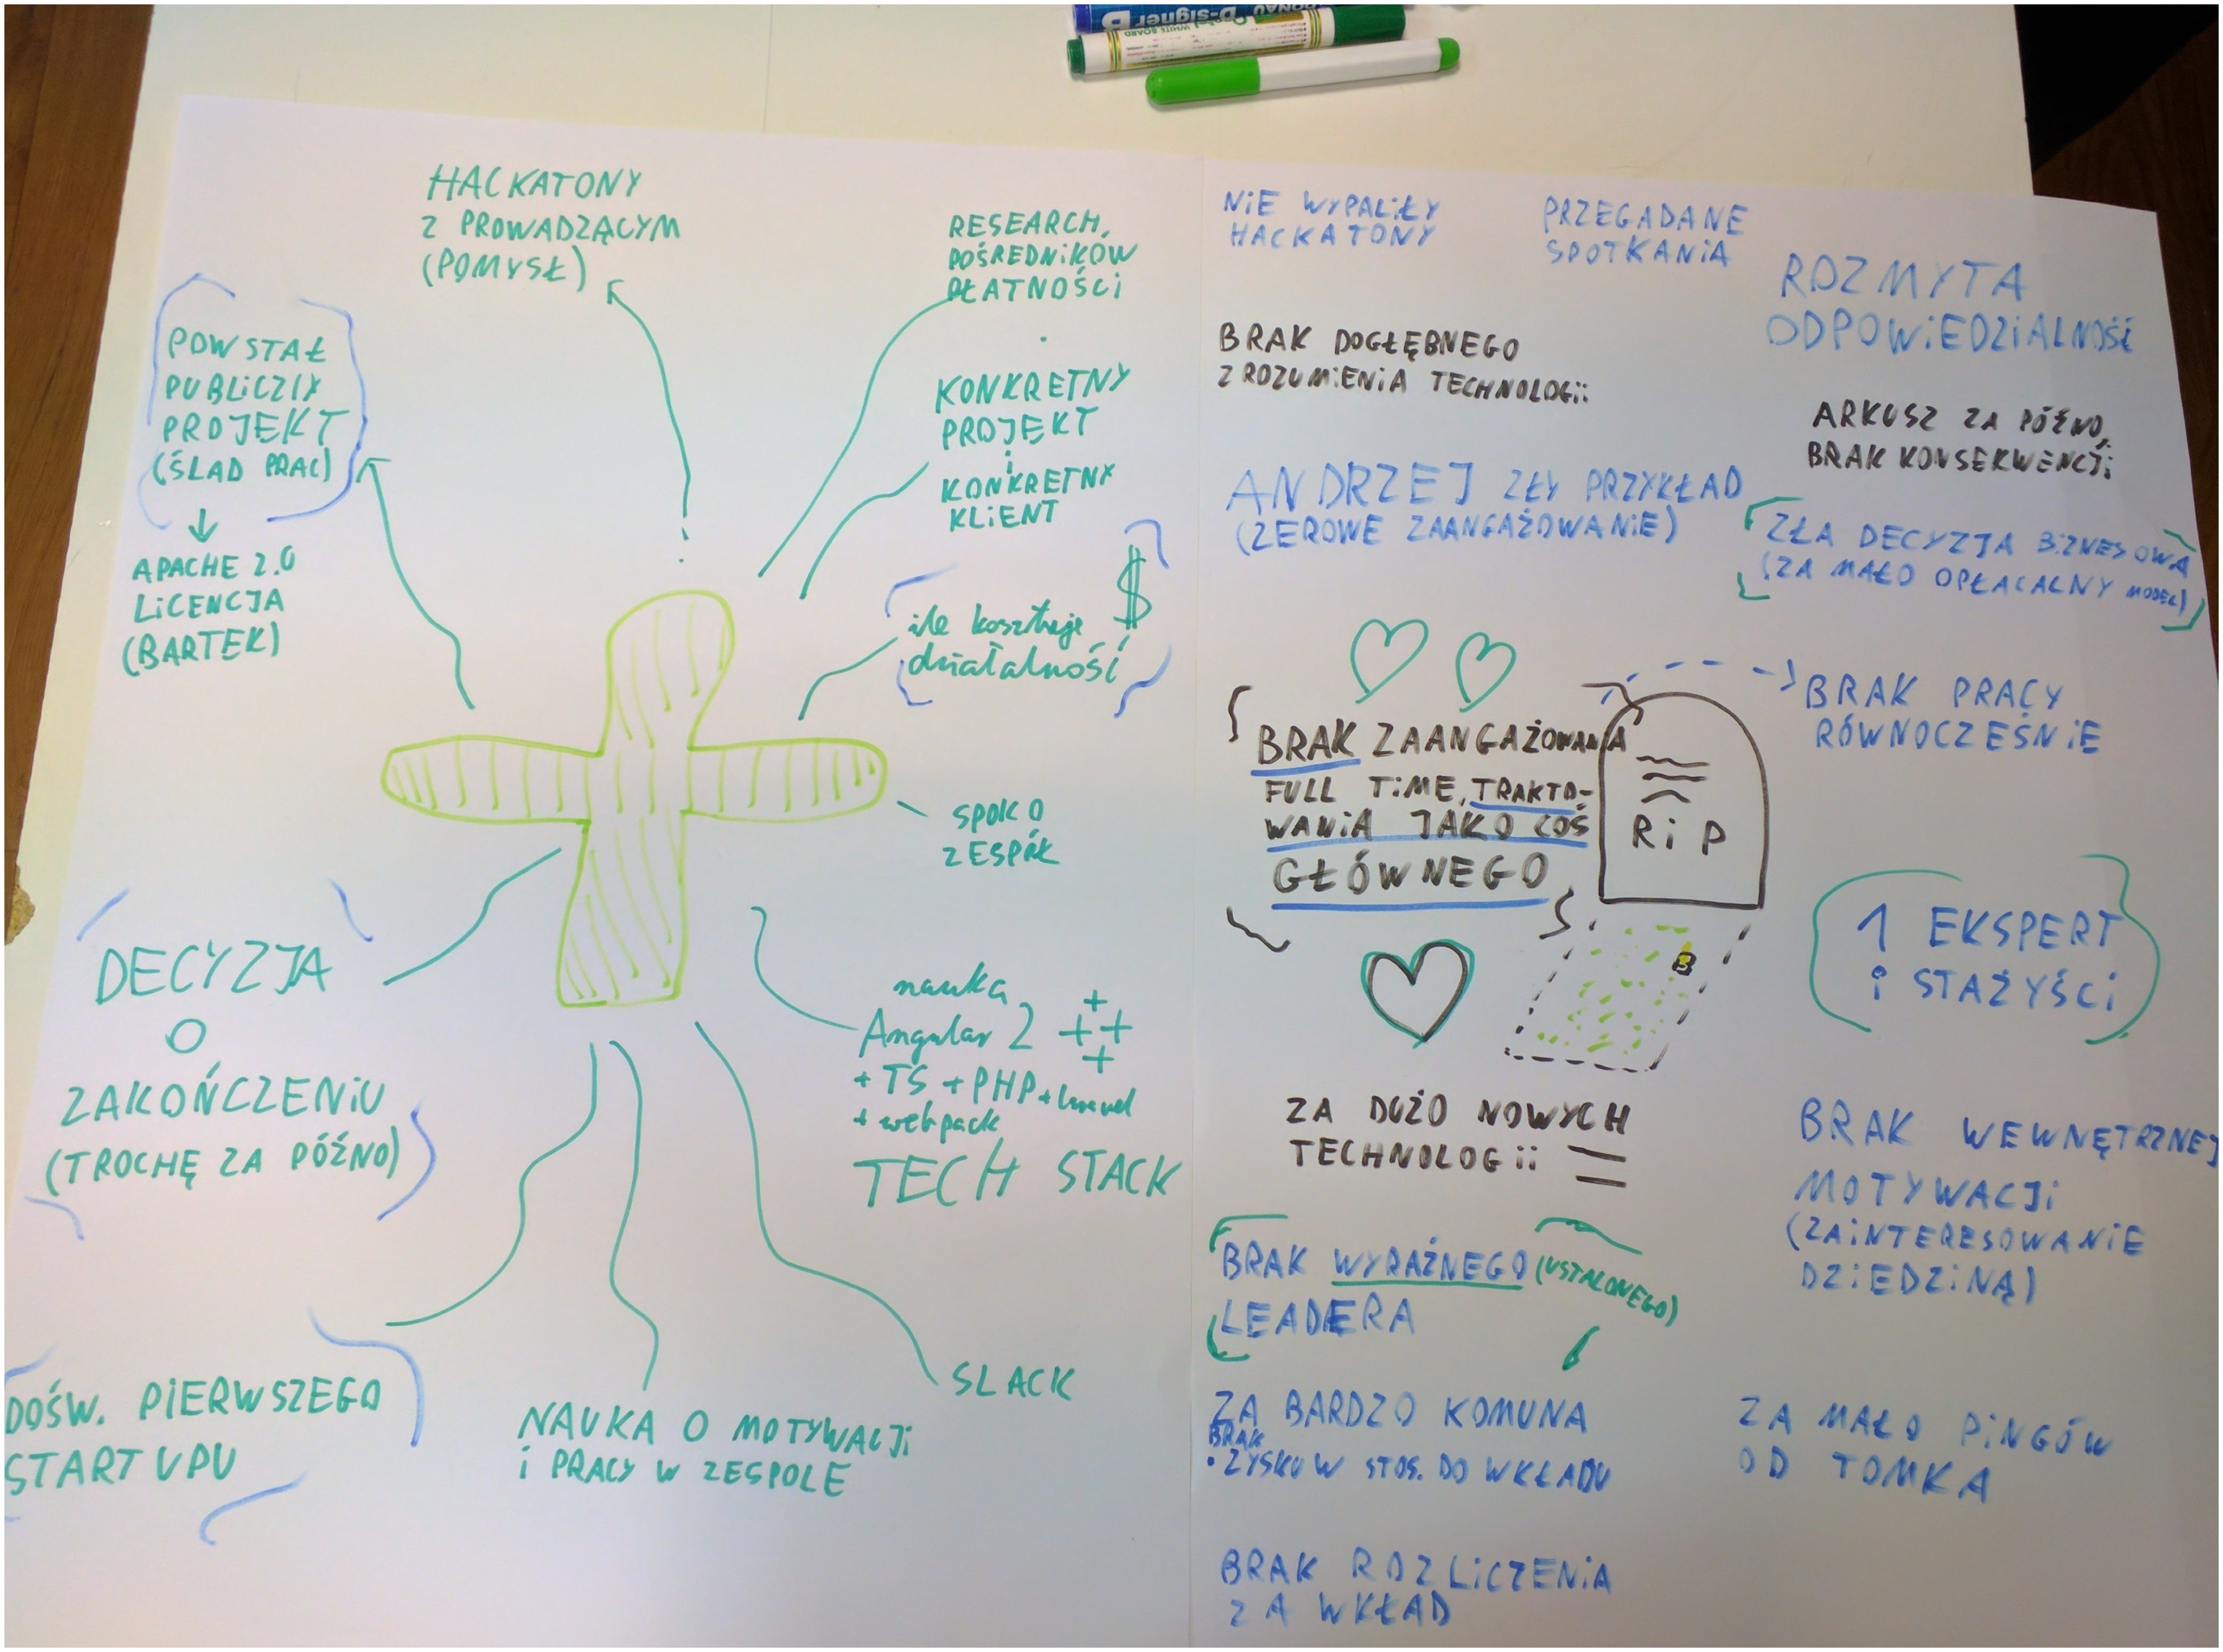
\includegraphics[width=\textwidth]{dncr-funeral}
    \caption{The DNCR project summary made collaboratively by the whole team during the meeting when the decision was made to discontinue the project}
    \label{fig:dncr-funeral}
\end{figure}
\FloatBarrier

\subsubsection{What Went Well: The Project's Successes}

Among the positive aspects of the project the team listed:
\begin{itemize}
\item Technology stack - although many team members did not manage to become productive in it, it was a drastically different experience from what most of them did daily at work and it allowed them to learn a lot.
\item The first startup experience – as it often takes several failed attempts before a successful one.
\item Learning about many legal and financial aspects: how much it costs to sustain a private firm, how much it costs to start a limited liability company and what the best options are when using online payments intermediaries.
\item A swift, albeit coming slightly too late, decision to end the project, when it became clear it would not lead anywhere. Also the fact that the project was rather well defined and had a client from the start, so the initial objectives of the project were clear.
\item The team enjoyed collaborating together and working on the project outside paid work allowed them to learn a lot about aspects of team motivation. The team appreciated various methods that were attempted to make the collaboration work (retrospectives, idea for guided hackatons, work logging and others)
\item Open-sourcing the project, which leaves a public trace of the performed work, which can be very useful, i.e. it can be added to CVs.
\end{itemize}

\subsubsection{What Made the Project Fail}
The team found the following reasons for the project's failure:
\begin{itemize}
\item The most important reason was that most team members did not treat the project as the "main thing" they needed to focus on. On the one hand, it was hard to expect several people to suddenly resign from their work and spend all their efforts on a project that might or might not succeed and might or might not return the invested time and money; on the other hand, if something is not given an absolute priority, then naturally regular work and other aspects of life will at times consume most of the attention and commitment and a side project will plummet. And with very little time spent on the project, very few mistakes could be made in order to still have a chance for success.
\item Overwhelming technologies and "one expert surrounded by interns" situation. It is natural to learn new languages, frameworks and tools in software development, but launching into two completely unfamiliar technology stacks, especially if one of them was the front-end development, which in recent years became quite daunting for newcomers, especially working part-time, was proven to be too hard for most team members. Another aspect of technological shortcomings was the usage of Docker in development environment, which in theory worked on all platforms, but in practice broke constantly with new versions for team-members working on Windows. Overall, as was stated during the meeting, "the lack of in-depth technology understanding" naturally resulting from lack of experience with technology slowed most of team-members down tremendously.
\item The next critical aspect was about the way the team organized work. During the project kick-off meeting, the team decided that despite different skill-sets (one experienced developer) and different amount of time dedicated to the project (only one developer worked on the DNCR full time), work of every member would be treated equally in the light of future financial gains. On top of that, there was no clear leader elected, so instead of an enthusiastic, collaborative atmosphere, the team members demonstrated a sociological phenomenon called the diffusion of responsibility.
\item The diffusion of responsibility was amplified by an absolute lack of consequences towards underperformers. Out of the seven initial members, one resigned early and two others practically did not contribute anything during the course of the entire undertaking. One other member was active mostly in the first phase of the project. As a result only three people worked for the declared amount of time, and the apparent lack of engagement from others only lowered morale and enthusiasm of the active members. 
\item The lack of intrinsic motivation was another aspect of low commitment among team members. Only one member knew the client directly and felt close to the domain and emotionally invested in making the project succeed, others had a colder, business- oriented attitude. Since there was no team leader, these members felt they were not held accountable for not keeping the constant commitment.
\item Many team members confessed to becoming discouraged over time and no longer fully convinced by the initial idea of the business model, claiming that the number of dance schools on the market was not sufficient to financially return the investment any time soon and that bringing the application to other domains or creating a platform for dance class attendees seemed to be unattainable in the near future.
\item Another set of drawbacks was that many ideas to improve team workflow were not successful: the guided hackatons did not take place after all, the work log was introduced too late and meetings were mostly about business and discussion, not about the coding sessions. The lack of regular work space was in itself viewed as an important aspect; it made it harder for underperformers to gain traction (and easier to keep underperforming) and it made the collaboration, especially code reviews, much more time consuming.
\end{itemize}

\subsection{The Case Study Results}
\label{sec:research-questions}
A few months later, when researching the present study, I became acquainted with literature on the subject in an attempt to gain a deeper understanding not only of the reasons why the project failed, but also of what could have been done differently. What other approaches could facilitate a better collaboration and improve the chances of success of future projects and what guidelines could be prescribed for other startups? And so, with the benefit of hindsight, the following is an attempt to address the previously raised research questions.


\subsubsection{RQ1: What Lean UX practices are most important in beginning phases of startup?}
Early stages of startup activities revolve mainly around validating problem, market and the product \citep{klein2013ux}. DNCR team did quite well in that regard, performing both qualitative and quantitative market research and by doing competitive product audits. On top of that, design of the product was validated with client using interactive prototype. All these activities gave the team necessary confidence in initial direction of action.

Of course there was room for improvement - hypothesis that customers would want to search for dance courses and pay for their classes online was critical for product future, yet instead of performing semi-statistically significant (40 respondents) online survey, it would be better to follow \cite{blank2013four} advice of Getting Out Of the Building (GOOB) and just go to several dance courses and perform survey in person, so follow-up questions could be asked, which would be a much better way to validate the idea.

Furthermore, more dance schools should be collaborated with from initial phases of the project, so solution the team would arrive to would be more universal and not just a perfect fit for the first client. The team was well aware of that, but planned to acquire new clients after initial MVP version, which unfortunately didn't work well as the team failed to finish the MVP.

The general advice for startups is then to:
\begin{itemize}
\item Actually perform various types of research and design validation before starting implementation, as it allows to clearly set initial direction
\item Especially in the beginning, focus on in-person, qualitative surveys. Quantitative research has it's many uses, but as \cite{klein2013ux} notes, online surveys cannot be considered as being in touch with users.
\item Competitive products audits cannot be recommended enough. They let the team learn from mistakes of others and in case of EU markets, often very similar solution already exists abroad (especially in US) an can serve as great source of inspiration.
\end{itemize}

\subsubsection{RQ2: How can Lean UX practices influence Minimal Viable Product building and what are the impediments in adopting them?}
As for implementation, Lean UX, following Lean Startup, advises treating each feature as a hypothesis to be tested and considered done only once proved to improve business metrics, usually via quantitative A/B testing. This can be hard at early implementation stages, when there is neither infrastructure nor user base for such tests yet, so in order to start iterative build-measure-learn loop, the team has to swiftly create Minimal Viable Product. It's important to note that Lean UX doesn't really discuss or define practices for MVP building, it generally embraces Agile and assumes the engineers will do the right thing. \cite{klein2013ux} discusses how hard is it to choose just the most necessary features at the beginning.

And this is where DNCR team failed hard. Initial design vision and "minimal feature-set" was ridiculously misaligned with the team's skill-set and it was noticed much too late in the process. As a result, after more than 4 months focused solely on implementation in team of 6 developers, the MVP still wasn't officially finished. \cite{ries2011lean} addresses this in his case study of actions by David Binetti, the CEO of Votizen, platform for civic participation in political process:
\begin{quote}
Votizen story exhibits some common patterns. One of the most important to note is the acceleration of MVPs. The first MVP took eight months, the next four months, then three, then one. Each time David was able to validate or refute his hypothesis faster than before. 
\end{quote}
Ries then argues that it's not due to Binetti previous product development work, as it often was discarded across different MVPs. It was partly due to existing testing infrastructure, but it was mostly due to "hard-won lessons David had learned through each milestone".

So it's not only the DNCR team that misunderstood the minimalism intended by MVP. In particular, the team needlessly focused on correct design scaling based on resolution - mobile first approach is a great guideline, but it just wasn't needed at this point in time. Moreover, team members were too strict in code review process - good code is important, but when reviews take long weeks and slows feature development, then it's a waste of effort. When learning new technology it's okay to have code of less quality and improve in the process. It's infinitely better to have validated product ridden with technological debt than to have amazing code that didn't reach the market or even validation phase. Ideally, it's great to have both, but sometimes the choice has to be made.

Thus, general advice for startups regarding MVP is to:
\begin{itemize}
\item Consider team's skill-set and other performance risks when determining feature-set of an MVP. It's main role is to quickly enable build-measure-learn loop and until it starts, the team doesn't really learn anything about their product.
\item Prioritize, prioritize, prioritize, as sometimes too much emphasis on good development practices is a waste of effort. \cite{klein2013ux} even proposes to put off visual design at first, as it is both faster to iterate and it doesn't influence interaction testing.
\item Consider MVP to be more of a prototype than a product. MVP has to be viable, but the minimal part is really important - if developers don't feel shame about lack of features of released version, or worse, haven't released any version few months into development, then this is not an MVP they're building.
\end{itemize}

\subsubsection{RQ3: What are the key challenges in startups regarding technology?}
This question is very hard to answer other than "it depends", as every startup faces different technological challenges.

Firstly, it's important to really understand consequences of technological choices. In DNCR project, choosing back-end technology language Ruby was considered and eventually PHP was chosen despite the fact that most of the team had extensive experience in Java. Of course it's true that Java servers cost more and of course it's tedious to always use the same language and technology, but startups really provide enough novelty outside of technology and cost of leaving familiar technology stack for new one is really not to be underestimated. As almost all members were also new to front-end development, instead of being productive at least in server-side aspects from day one, many members failed to become productive at all during the project.

Secondly, in principle it's great to have whole development team consisting of only full-stack developers, it doesn't unnecessarily split the team and every member has autonomy to implement full business features on their own. In practice, it resulted in low granularity tasks that took weeks to implement and additional weeks to review.

Moreover, Docker as a tool of abstracting over developer environment is great in theory, but in practice it made three Windows 10 developers' lives in the team miserable, crashing constantly in hard to debug ways. Two of them switched to Linux Virtual Machines and one suffered with broken environment after each update to the end of project. Additionally, development environment facilitating Docker prevented the team from being able to use Angular HMR (Hot Module Reloading), which would make development feedback loop even tighter.

Another aspect was decision to use Release Candidate (RC) version of Google's Angular, before it's 2.0 release. In theory release candidates, made after alpha and beta, should be stable, but that was not the case. Angular upgrades around RC5 were painful, as Google team introduced significant breaking changes and updated their documentation which wasn't versioned before 2.0 and DNCR team couldn't upgrade because of dependencies on earlier Angular RC versions. Thus for some time the team was out of sync with documentation.

Yet another aspect was implementing token authorization and in general user login handling. The team evaluated using COTS (Commercial Off-The-Shelf) solution, offering Social Sign-In for free until certain user limit, but eventually the team decided to manually implement solution using JWT (JSON Web Tokens). Again, in this case it would've been a better choice to just use COTS solution and worry later once product is validated and number of users approaches that limit.

The team, of course, did some things well too - one of them was to start implementation phase from extensive documentation about development environment setup, integration with IDE and configuration of Continuous Integration and so that important aspect went smoothly (this setup documentation is available at \url{https://github.com/tlegutko/dncr}). Usage of Docker was the only part that didn't go well.

Overall, general advice for startups regarding technology is to:
\begin{itemize}
\item Think twice before relying on Docker when using Windows
\item Above all, think ten times before choosing novelty of unfamiliar technologies and seriously consider its impact on team's productivity
\item Full-stack development team is nice, but consider that an end-goal, not a requirement from day one. It's okay to specialize in the beginning. And remember to keep high enough granularity of tasks.
\end{itemize}

\subsubsection{RQ4: What are the factors that impact the success of startups regarding team?}
As mentioned during project retrospective, the team suffered from diffusion of responsibility due to underperformers and lack of leadership.

Regarding leadership, the team had three candidates: leader of team at work where most developers collaborated prior to project, developer who brought the idea along with the client and organized team's work and the only developer experienced with technologies, who was also responsible for design. The first one wasn't very committed from the start, while the second and the third thought the other one was more fitting. The end scenario was worst possible, as no one was selected and it negatively affected perceived responsibility of team members.

Lack of formal definition of startup \citep{paternoster2014software} was another reason for lack of leadership and even distribution of costs - one of leader candidates perceived a startup as a collaborative, passionate effort where there is no need for formal structure and everyone gives their all. As \cite{giardino2014early} notice:
\begin{quote}
  One of the key determinants of success in startup companies is the passionate behavior of the founders. People who lack passion often use the first barrier they encounter as an excuse for failure. People who have high passion will do whatever it takes to overcome these barriers.
\end{quote}

This assumption was part of the reason that underperformers' behavior was accepted for so long. Initially no formal structures were assumed to be necessary, as team was doing well on initial motivation from starting the project. Furthermore, initial lack of productivity was expected due to lack of experience with technology. What was noticed much too late was the fact that the lack of productivity was not due to hardships in mastering technology, it was due to not spending time on the project. Work logging and simple performance evaluation like weekly summary should have been introduced and acted on earlier.

Moreover, the team lacked regular face-to-face collaboration, especially during implementation. Even though it's one of main principles listed in Agile Manifesto, the team failed to incorporate it. Of course it's hard to coordinate 6 people, mainly working after regular work hours, of course it's more convenient and flexible for developers to work remotely when it fits them most. But the truth is, if the team is inexperienced with technology, there is a high chance that this will not work. Firstly, every technological question and problem can either take longer when developer solves it himself or can be solved instantly with help of someone more experienced. The former is of course necessary for effective, long term learning, but lack of balance between the too is of huge impact for productivity. Secondly, all discussions, especially over code review, take much longer. And unproductive loneliness takes high toll on motivation.

Advice for startups regarding social/people/team aspect is to:
\begin{itemize}
\item Explicitly choose leaders. Choosing technological leader and team leader is a good choice in situation similar to DNCR project. Choosing another configuration is also good, as long as roles are clearly defined.
\item Although both methodological and technological advancements made startups much less risky, they still require passionate founders who will persevere and overcame all eventual roadblocks.
\item Underperformers should be moved away from the team quickly. It may seem counter-intuitive, as extra developer seems to always push work a little bit forward, but when his contribution is minimal, slows the team down and negatively affects morale, it's the right thing to let them go.
\item Seriously consider the impact of abandoning regular collaborative implementation sessions and unless the team has experience working remotely in particular technology, think hard about counter-measures to save team's productivity.
\end{itemize}

\subsubsection{RQ5: Which Lean UX practices can be used in startups regarding business/market?}
DNCR project was targeting dance schools, but in the next stages the plan was to also target customers and create two cooperating products, which would allow people to search and compare dance courses across different dance schools. This cooperation would bring various benefits, as data for customers would always be up-to-date as schools would use their products daily to manage their business procedures. Moreover, customers searching for dance courses would create advertising opportunity for dance schools and let them target precisely selected group of potentially interested clients.

In fact, in late stages of project, the team started to wonder if the development was started from the right product. That is, validating product for business is harder than validating product for customers, as there is naturally much less companies than clients these companies target. Moreover, in order to convince companies to consider spending significant sum of money on product, it has to offer some convincing initial feature-set. And as DNCR project was trying to achieve it, it spent several months implementing features, but not learning anything about their solution's viability on the market.

There was idea to pivot into creating platform for clients, with idea for validating it presented briefly on Figure \ref{fig:znajdz-taniec}. It would be really easy to implement and \cite{klein2013ux} advices exactly these type of tests at the beginning of the project. This way, spending reasonable amount of money on Google AdWords and Facebook Ads, the team could easily get the idea about number of potentially interested customers and thus answer one of the most important hypotheses in their project.

But the downside was that as project progressed really slowly, it seemed unwise to split attention to two products. It was tempting to abandon initial product for dance schools for the time being and shift attention to platform for clients, but having not yet validated product for dance schools, it would seem to be tremendous waste to drop it, because who knows, maybe it was the right approach? The team didn't have any data to scientifically make the decision, they waited too long to start measuring and learning loop.

\begin{figure}[h]
    \centering
    
\includegraphics[width=0.7\textwidth]{znajdz-taniec}
    \caption{Idea for validating platform for clients with two-page prototype. On first screen there would be Google-like search bar with question "Do you want to dance?" and once user performs his search, results page with mocked data shows up. Below it appears window informing about site being a prototype in development and asking for email to be notified once site launches.}
    \label{fig:znajdz-taniec} 
\end{figure}

Advice for startups regarding business/market is to:
\begin{itemize}
\item Embrace the idea of smoke tests, where product is launched, pretending to "not work yet", with the sole intent on validating the idea before spending months on implementation.
\item Producing MVP for businesses can be harder and more time consuming than creating MVP for clients.
\item It's of utmost importance for a startup to find the quickest possible way to learn whether their product answers the market needs.
\item Read Eric Ries' book \textit{The Lean Startup} \citep{ries2011lean}, it's main focus is on business/market aspect and it features multiple case studies discussing variety of approaches.
\end{itemize}

\subsubsection{RQ6: How are success factors in Agile projects \citep{cao2008agile} applicable to startups?}
\citeauthor{cao2008agile} list 6 success factors, presented from most to least significant: delivery strategy, Agile software engineering techniques, team capability, project management process, team environment and customer involvement. All of these factors are further divided into attributes representing desired activity, i.e. "regular delivery of software" or "delivering most important features first".

DNCR project suffered from shortcomings in all of these aspects:
\begin{itemize}
\item The team was so focused on achieving feature-rich MVP that it neglected regular delivery and as a result did not learn during MVP implementation phase
\item The team failed to choose simplest design and architectural solutions, coding standard emerged quite late in the process.
\item Team capability left much to be desired, both technological and motivation-wise
\item Ad-hoc project management with lack of leadership, lack of individual progress tracking and no consequences towards underperformers
\item Team was not collocated and it negatively impacted team's performance
\item Relationship with customer and customer commitment were pretty mediocre. After design validation, the next meeting was supposed to be with MVP, but as MVP was falling behind the schedule, there was no intervention from either of the sides
\end{itemize}

Advice for startups regarding success factors in Agile software projects identified by Chow and Cao is to:
\begin{itemize}
\item Keep working on "Agile and basics". Adopting modern methodology such as Lean Startup or Lean UX is by no means an excuse to neglect many development practices that these methodologies just do not explicitly focus on.
\end{itemize}

\subsubsection{DNCR project was not the only one with these problems}
As it is often the case, DNCR team was not alone in their struggles and resulting failure. This study results align well with results from other works.

Giardino, Wang and Abrahamsson \citep{giardino2014early} performed case studies of two failed startups. Both of them released the product, but didn't attract customers. Similarly to DNCR project, these startups neglected learning during implementation phase and missed entrepreneurial characteristics in team members, leading to lack of motivation and decreasing commitment. Business-side, they were preoccupied with profitable business model instead of solving problem/solution fit and learning from customers. They were "addressing specific challenges in the wrong time". And same as DNCR team, instead of a close collaboration with their clients, they were too absorbed in technology.

\cite{may2012applying}, describing her failed startup argues that single most important lesson was to learn to constantly test every assumption in order to keep progressing in the right direction. Among other reasons for failure she also notes not-thought-out technological choices, mainly about choosing bleeding-edge frameworks and failing to fire underperformers fast. these exact factors sound very similar to challenges faced in DNCR project.

Among key qualities needed for startup survival, \citeauthor{may2012applying} listed extraordinary passion, perseverance "and a lot of fast learning and smart decision-making". In DNCR project there was definitely not enough of these, but it's a real shame that the team didn't have that knowledge about problems of other startups during their own struggle. This is why it's very important to keep filling the gap in literature about startups, so new teams can find help and guidance more easily.

\subsubsection{Balancing learning and productivity}
The team learned Lean Startup and Lean UX methodologies as they progressed with the project, which meant that even though team members were aware of practices in theory, in practice they truly understood them only after learning from their own mistakes.

As for almost every member on the team DNCR was their first startup, lack of experience lead the team members to great learning opportunity about various aspects of startup activity including legal, financial and marketing aspects, not to mention new technologies. But the difference between learning and performing has to bee noticed, as it's absolutely unrealistic to expect to achieve business goals on absolutely unfamiliar grounds where everything is a learning experience, especially with limited time and resources. Balance needs to be maintained between the two and it often may lead to tough development decisions of accepting technological debt and use whatever is familiar to maintain momentum.

But in startups, with limited time and resources, there are only so many mistakes that can be made before project fails and it's paramount to be able to constantly focus on what's most important.

\section{Conclusion}
In this thesis, Lean UX practices in startups were studied from both theoretical and practical point of view.

First, Lean UX was introduced with historical view at methodologies it originated from - Agile, User-Centered Design and Lean Startup. these methodologies were briefly introduced and state of the art was discussed with special emphasis on attempts to combine these methodologies. There is surprisingly little research on startups in general and hardly any research on Lean UX and filling the missing gap was main motivation for this thesis.

Next chapters focused on case study of author's failed startup DNCR, active between 22.06.2016-01.12-2016. The goal was to analyze actions and decisions made by the DNCR team in light of approach proposed in literature and to provide lessons learned. Answers to research questions resulted in 18 guidelines for startups.

Most notable limitation of the study was that DNCR startup didn't reach the market and didn't even finish building MVP, thus many Lean UX practices for verified quantitative learning weren't performed and analysis focused on early-stage startup activities.

\subsection{Future work}
Above all, startups need more researchers' attention. In recent years books about startups targeted at entrepreneurs started to appear and that's a good thing, but there needs to be more systematic studies and especially experience reports and lessons learned, as they can provide guidance for many startups to come.

Moreover, software startups are definitely not only about software, but also about legal aspects, acquiring funding, marketing and so on - it's still remains to be explored in literature.

Furthermore, Lean Startup and Lean UX are not very verbose about engineering aspects and challenges of building either MVP or infrastructure allowing for A/B metrics. As these methodologies become more and more popular, hopefully these technological questions are to be answered soon.

\listoffigures
\bibliography{masters-thesis} 
\end{document}